\documentclass[twoside,12pt]{article}

\usepackage{lmodern}
\usepackage[T1]{fontenc}
\usepackage[spanish,activeacute]{babel}
\usepackage{mathtools}
\usepackage{graphicx}
\usepackage[inner=3.0cm,top=2.5cm,outer=2.0cm,bottom=2.5cm]{geometry}  
\usepackage{fancyhdr}
\usepackage{hyperref}
\usepackage{multicol}

\usepackage{glossaries}


\pagenumbering{gobble}
%\renewcommand{\baselinestretch}{1.5}
\usepackage{setspace}
\onehalfspacing

\setlength{\footskip}{42pt}

\title{\begin{center} 

\includegraphics[width=0.8\textwidth]{images/upc-logo.png} 
\end{center} 
\vspace{0.5cm} 
Proyecto Final de Carrera\\
INGENIER\'IA INDUSTRIAL \\
\vspace{0.5cm} 
\Huge{
RosPiBot}
\vspace{0.5cm} \\
 Memoria}

\author{}
\date{} % void to avoid put current date
\pagestyle{fancy}

\fancyhead[LO,RE]{\title{RosPiBot}}
\fancyhead[LE,RO]{\thepage}
\fancyfoot[LE,RO]{
\includegraphics[scale=0.5]{images/etseib-logo.png}}
\fancyfoot[C]{}
%\headrulewidth 0.4pt
%\footrulewidth 0 pt

%\makeglossaries
%\newacronym{IIC}{I$^{2}$C}{Inter-Integrated Circuit}
%\newacronym{SPI}{SPI}{Serial Protocol Interface}
%\newglossaryentry{electrolyte}{name=electrolyte, description={solution able to conduct electric current}}

\begin{document}
%\pagestyle{empty} 

\maketitle
\begin{center}
\large{$\begin{array}{ll}
\mbox{Autor:} & \mbox{Joan Guasch Iglesias} \\
\mbox{Director:} & \mbox{Manel Velasco Garcia} \\
\mbox{Convocatoria:} & \mbox{Fecha a presentar}
\end{array}$}\\ 
\vspace{2cm} 
\Large{Escuela T'ecnica Superior de Ingenier'ia Industrial de Barcelona}\\ 
\vspace{1cm}

\includegraphics[scale=1]{images/etseib-logo.png}
\end{center}
\thispagestyle{empty}
\newpage

\thispagestyle{empty}
\paragraph*{}
\newpage

%\thispagestyle{empty}
%\pagenumber{1}
\pagenumbering{arabic}
\fancyhead[LE,RO]{1} 

\normalsize
\begin{abstract}
Este proyecto consiste en el aprovechamiento de la plataforma rob'otica comercial WifiBot que corre el riesgo de quedarse obsoleta y rescatarla de su destino. Para ello se hace uso de una Raspberry Pi, un ordenador de placa reducida que ha revolucionado el mundo de la automatizaci'on desde el d'ia de su aparici'on en el 2012, como unidad de procesamiento de la nueva plataforma y que est'a basada en Linux. En el apartado de software, adem'as de incorporar herramientas que faciliten el trabajo a futuros usuarios se ha configurado para poder trabajar con ROS, una infrastructura digital para el desarrollo de software de robots creada por Willow Garage y extensamente utilizada en este sector.\\

A lo largo de este documento se exponen el estado inicial del robot, los nuevos requerimientos a cumplir, las modificaciones efectuadas incluyendo las complicaciones encontradas a lo largo del proyecto y el resultado final obtenido. Haciendo especial hincapi'e en el desarrollo de soluciones para cumplir los objetivos del proyecto, tales como el dise'no de circuitos electr'onicos, la integraci'on de los nuevos componentes o la creaci'on de una mejor interf'icie para el usuario. \\

\end{abstract}

%\thispagestyle{empty}
\newpage

\paragraph*{}
\thispagestyle{empty}
\newpage

\fancyhead[LE,RO]{3}
\tableofcontents
\setcounter{page}{1}
\addtocontents{toc}{~\hfill\textbf{P'agina}\par}
\addcontentsline{toc}{section}{Resumen}
%\setcounter{page}{1}
\addcontentsline{toc}{section}{Glosario}
%\setcounter{page}{4}
\fancyhead[LE,RO]{4}
%\setcounter{page}{3}
%\addcontentsline{toc}{section}{'Indice}
\newpage

%\pagenumbering{arabic}
\setcounter{page}{5}
\fancyhead[LE,RO]{\thepage}

\section*{Glosario}
\begin{description}
\item[UART] Universal Asynchronous Receiver-Transmitter
\item[SPI] Serial Protocol Interface
\item[I${2}$C] Inter-Integrated Circuit
\item[ADC] Analog to Digital Converter
\item[SoC] System on a Chip
\item[CPU] Central Processing Unit
\item[GPU] Graphics Processing Unit
\item[RAM] Random Access Memory
\item[RCA] Random Access Memory
\item[HDMI] Random Access Memory
\item[DSI] Random Access Memory
\item[CSI] Random Access Memory
\item[GPIO] Random Access Memory
\item[SD] Random Access Memory
\end{description}

%\printglossaries


\newpage

\section{Introducci'on}

\subsection{Estado del arte}

\subsection{Alcance}


\subsection{Objetivos}

\newpage

\section{Descripci'on }

\subsection{WifiBot}
\textbf{Wifibot} es una plataforma rob'otica, desarrollada por la empresa francesa \textbf{Nexter Robotics}, dise'nada para poder navegar en m'ultiples escenarios gracias a su dise'no. Su sistema de tracci'on a las cuatro ruedas, dise'no reducido y bajo peso, le otorga una gran flexibilidad.

\subsubsection{Caracter'isticas}
Este proyecto parte del modelo \textbf{WifiBot 4G}, producido durante el periodo 2002--2006 y que a grandes rasgos incluye::

\begin{figure}[ht]
\centering
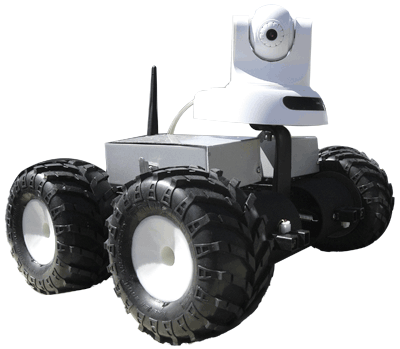
\includegraphics[scale=0.5]{images/Visuel_Wifibot_2.png} 
\caption{Wifi Bot 4G}
\label{fig:Wifi Bot 4G}
\end{figure}

\paragraph*{}

\begin{multicols}{2}
\begin{itemize}
\item CPU:
	\begin{itemize}
	\item Procesador AMD Au1500
	\item 400MHz
	\item Mem'oria RAM de 64MB
	\item Mem'oria Flash de 32MB
	\end{itemize}
\item Interf'icies:
	\begin{itemize}
	\item 4x Ethernet 10/100
	\item 1x USB
	\item 1x I$^{2}$C %\gls{IIC}
	\item 1x RS232
	\end{itemize}
\item WIFI:
	\begin{itemize}
	\item WiFi con est'andar 802.11a/b/g
	\item Modos Access Point, Bridge, Client y Router
	\item 1x Antena de 5dBi
	\end{itemize}
\item Sensores:
	\begin{itemize}
	\item 1x C'amara IP
	\item 2x Sensor IR de dist'ancia
	\item 2x Codificador de efecto Hall (Hall Encoder) 
	\item 2x DSPIC30F2010
	\item 1x Nivel de bater'ia
	\end{itemize}
\item Motores:
	\begin{itemize}
	\item 4x Motor de 7.2V
	\item Reductora $i=50:1$
	\item Par nominal 8.87Kg/cm
	\item Velocidad nominal 120Rpm
	\end{itemize}
\item Dimensiones:
	\begin{itemize}
	\item Longitud 28cm
	\item Anchura 30cm
	\item Altura 20cm
	\item Peso 4.5Kg
	\end{itemize}
\item Bater'ias:
	\begin{itemize}
	\item 9.6V NiMh (8 celdas)
	\item Capacidad 9500mAh
	\item Autonom'ia de 2 horas
	\end{itemize}
\end{itemize}
\end{multicols}

\subsubsection{Estructura}

La estructura de la base est'a formada por dos secciones sim'etricas que llamaremos hemisferios izquierdo y derecho. Estas dos partes est'an unidas por una barra roscada que atraviesa transversalmente todo el robot, ofreciendo un eje de rotaci'on entre los dos elementos, cualidad que le otorga una mayor adaptaci'on a superf'icies irregulares.
%include image SolidWorks
%como vemos en figura \ref{fig:Wifi Bot 4G}

\subsubsection{Estado Inicial}  
La plataforma de la que se dispon'ia en un principio carec'ia de cierta cualidades. La m'as destacable era la inestabilidad de la red WiFi, dicha conexi'on sufr'ia constantes ca'idas con lo que dificultaba enormemente su teleopraci'on. Su otro tal'on de Aquiles era su escasa documentaci'on disponible, al ser un producto que su fabricante da por descontinuado y al no disponer de una comunidad que lo mantenga, dicha base rob'otica provocaba quebraderos de cabeza para usuarios noveles. Finalmente, las bater'ias al haber completado su vida 'util, dispon'ian de una carga efectiva muy inferior a la inicial. En cambio, tanto la estructura, ruedas, motores y sensores se encontraban en mejores condiciones\\
\newpage

\subsection{Raspberry Pi}
Raspberry Pi es un ordenador del tama'no de una tarjeta de cr'edito desarrolado en Reino Unido por la \textbf{Raspberry Pi Foundation} con el objetivo de fomentar las bases de la computaci'on en escuelas. El desarrollo de este diminuto ordenador empez'o en el 2006 hasta alcanzar su madurez y comercializaci'on en Febrero del 2012. 

\begin{figure}[ht]
\centering
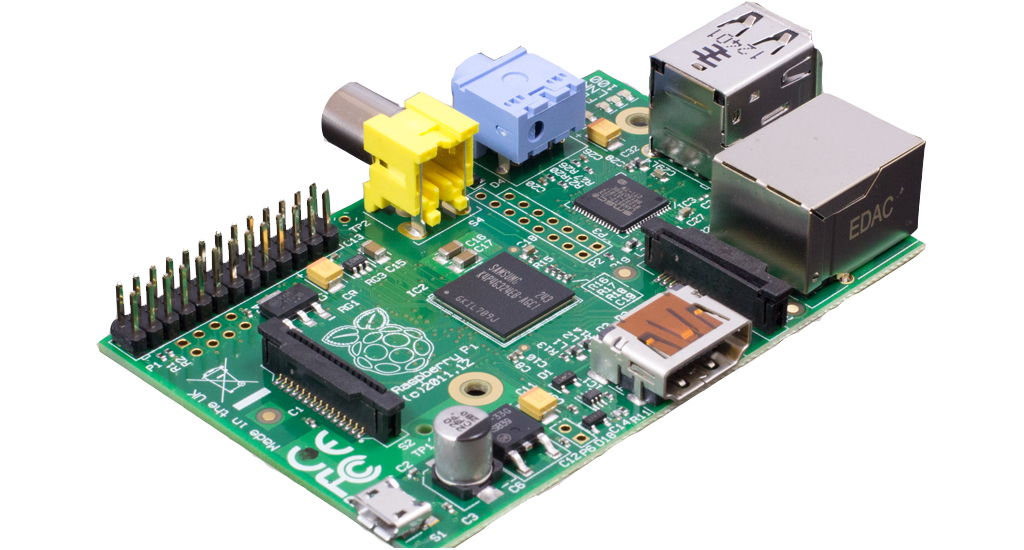
\includegraphics[scale=0.2]{images/raspi.png} 
\caption{Raspberri Pi}
\label{fig:Raspberry Pi}
\end{figure}

\subsubsection{Caracter'isticas}
Aunque existen varios modelos de Raspberry Pi, este proyecto se basa en el modelo B (segunda revisi'on). Este modelo se caracteriza por:

\begin{figure}[ht]
\centering
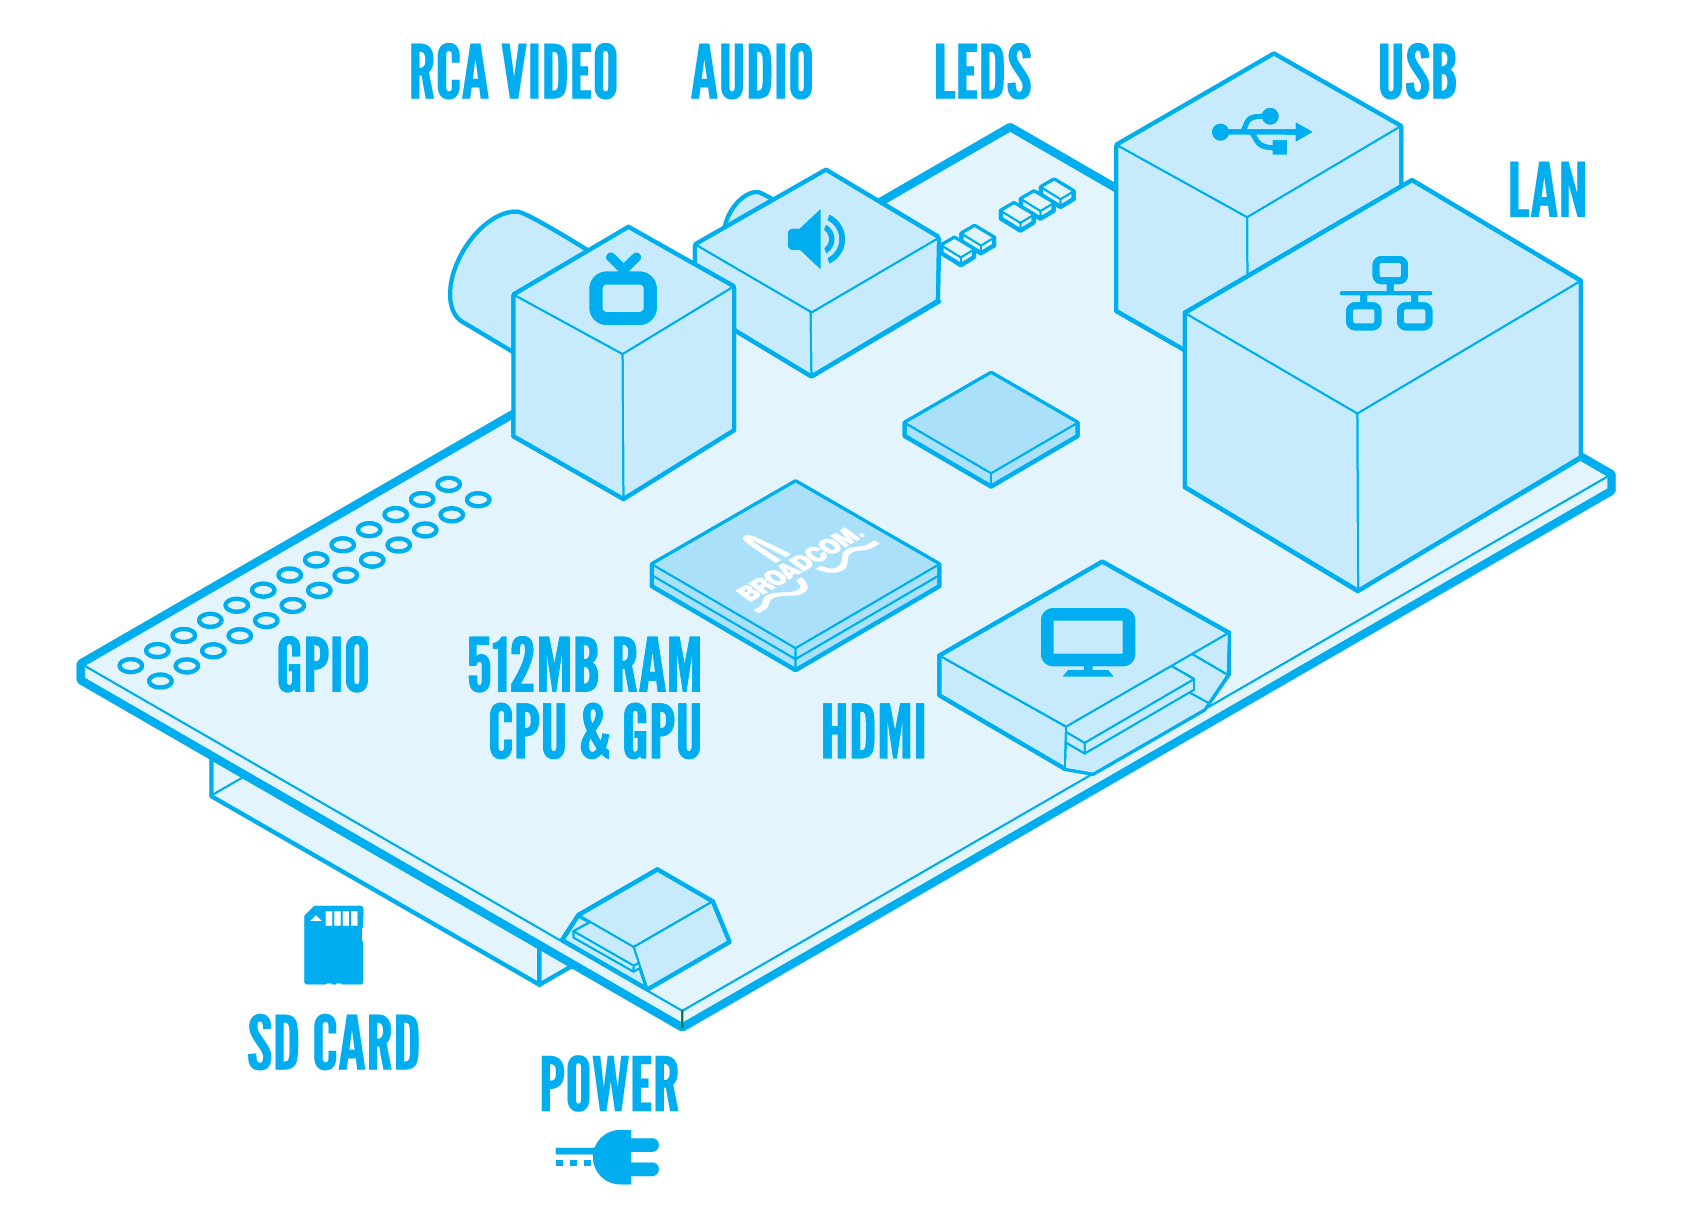
\includegraphics[scale=0.15]{images/RaspiModelB.png} 
\caption{Esquema Modelo B}
\label{fig:Esquema Modelo B}
\end{figure}

%\begin{multicols}{2}
\begin{itemize}
\item Procesador Broadcom BCM2835 (SoC) compuesto por:
	\begin{itemize}
	\item CPU: ARM1176JZF-S (Arquitectura ARM 11)
	\item GPU: VIDEOCORE IV (250 Mhz)
	\item Mem'oria RAM de 512MB
	\end{itemize}
\item Connexiones multimedia:
	\begin{itemize}
	\item 1x Entrada de v'ideo: CSI
	\item 3x Salidas de v'ideo: RCA, HDMI y DSI
	\item 2x Salida de audio: 3.5mm jack y HDMI
	\item 1x RS232
	\end{itemize}
\item Connexiones de datos:
	\begin{itemize}
	\item 1x Ranura tarjeta SD (Disco Duro)
	\item 2x Puertos USB 2.0
	\item 1x Puerto Ethernet RJ45 (10/100 MBit/s)
	\end{itemize}
\item Perif'ericos de bajo nivel:
	\begin{itemize}
	\item 8x GPIO
	\item 1x UART
	\item 1x I$^{2}$C bus
	\item 1x SPI bus (dos pines de selecci'on)
	\end{itemize}
\item Otros datos:
	\begin{itemize}
	\item Alimentaci'on: 5V via MicroUSB o GPIO
	\item Medidas: 85.6mm x 56mm
	\item Peso: 45 g
	\end{itemize}
\end{itemize}
%\end{multicols}



\newpage

\subsection{Protocolos de comunicaci'on}

\newpage

\section{Especificaciones}
Tal y como se ha definido anteriormente, el objetivo de este proyecto consiste en ofrecer una plataforma funcional para los futuros usuarios. Para definir esta ''funcionalidad'' se ha basado en el conocimiento aportado por antiguos usuarios, trabajadores en productos similares y en la experiencia propia. \\

Las especificaciones se han clasificado seg'un su or'igen. Dependiendo de si son de car'acter \textbf{software}, \textbf{electr'onico} o \textbf{mec'anico}. Las especificaciones de car'acter inform'atico engloban aspectos como la interf'icie con el usuario, las herramientas de desarrollo (librer'ias, documentaci'on) y la disponibilidad a futuras modificaciones. Por contra, la electr'onica ha de evitar que el usuario se encuentre obligado a manipular el interior del robot, pero que en el caso de dicha situaci'on permita una soluci'on simple del problema. Adem'as, la electr'onica ha de incorporar un sistema que permita conocer estados del robot de manera sencilla. Finalmente, la mec'anica se encarga de incorporar las nuevas especificaciones en la plataforma, manteniendo el concepto inicial. Igual que en la electr'onica, en el caso de una futura manipulaci'on por parte del usuario, el dise'no ha de facilitar el acceso a cualquier ubicaci'on.

\subsection{Software}
El principal requisito del software es ofrecer un acceso simple al usuario. Teniendo presente el hecho que pueda ser utilizado tanto para usuario noveles como para usuarios experimentados. Por ello se ha planteado las siguientes especificaciones.

\subsubsection{Web}
Se ofrecer'a un servidor web que permita de visualizar f'acilmente el estado del robot como por ejemplo: el nivel de carga de bater'ias, sensores de proximidad, velocidad de desplazamiento, consumo de motores, etc. Adem'as se incluir'a una pantalla d'onde se monitorizar'a una c'amara que incorpora el robot y un par de terminales de comandos.
En otro apartado de la web se ofrecer'a la descarga de todos aquellos documentos necesarios para el usuario, evitando as'i que el usuario pierda tiempo en la b'usqueda de la documentaci'on.

\subsubsection{Librer'ias}
%Por facilidad de uso y comodidad se ha decidido que todo el software utilizado en este proyecto se base en $Python^{ TM}$, un lenguaje de programación
Para aquel desarrollador que decida utilizar esta plataforma se le ofrecer'a un conjunto de librer'ias que permitan trabajar con el robot de manera comoda. Estas librer'ias se compondr'an de una sintaxis limpia y un c'odigo legible que proporcinar'a una f'acil interpretaci'on.    

\subsection{Electr'onica}
El objetivo de la electr'onica es ser la parte m'as vital de la plataforma, pero pasando desapercibida por el usuario. Ofreciendo una m'inima interacci'on pero suficiente para comprender el estado del robot. Esta interacci'on se har'a mediante se'nales luminosas o ac'usticas, e indicar'an los siguientes estados.

\subsubsection{Funcionamiento}
En la plataforma de partida no se dispone de ning'un medio que indique si se encuentra operativo, por ello la primera especificaci'on de la parte electr'onica ser'a la incoporaci'on de un se'nal luminosa que muestre si el robot est'a encendido o apagado. Tambi'en existe la posibilidad de ofrecer informaci'on de otros estados.

\subsubsection{Alimentaci'on}
Las bater'ias ofrecer'an  una autonom'ia suficiente para moverse en un entorno exterior, se estipula un m'inimo de 2 horas en movimiento como m'inimo aceptable. Adem'as de la duraci'on, su recarga deber'a de ser lo m'aximo de comodo para el usuario, evitando que tenga que manipular las celdas de energ'ia. Se recomienda elementos de seguridad ante problemas como sobrecargas o cortocircuitos y de gesti'on de energ'ia para aumentar la vida 'util.\\

Otro punto a tener en cuenta es la disponibilidad en encontrar repuestos de la bater'ia, por ello se usar'an productos comerciales f'aciles de adquirir. Finalmente, se monitorizar'a el nivel de carga a partir de unos elementos luminosos.

\subsubsection{L'ogica}
Para el control de la plataforma el proyecto se ha basa en uso de la Raspberry Pi. Dicho ordenador ser'a el responsable de efectuar todo los c'alculos y 'ordenes, A'un as'i, a causa de sus limitaciones se precisa de una l'ogica complementaria capaz de gestionar y contabilizar las lecturas anal'ogicas de los sensores, el control de motores, la comunicaci'on externa y la distribuci'on de energ'ia.

\subsubsection{Comunicaci'on}  
Para poder interaccionar con el plataforma rob'otica se proponen 3 medios alternativos. Cada uno de estos canales permitir'an el acceso al usuario. Un primer medio ser'a por via cableada, a partir de un cable de red, los otros dos ser'an por via inal'ambrica, por un lado se buscar'a un red Wi-Fi predefinida y por otro se crear'a una red Wi-Fi propia. 

\subsection{Mec'anica}
Se intentar'a en la medida de lo posible mantener la silueta caracter'istica del robot, asignando mayor prioridad a aquellas modificaciones motivadas por software o  electr'onica. 

\subsubsection{Estructura}
Se desea mantener la estructura b'asica de la plataforma, dejando su peculiar forma de dos bloques unidos por una barra roscada longitudinal. Se mantendr'a el concepto de perfiles cuadrados como elemento estructural pero modificando la separaci'on entre ellos.La ubicaci'on de los distintos elementos se dispondr'an seg'un su relaci'on con el resto de dispositivos, uniendo seg'un se traten de control de potencia, l'ogica o comunicaci'on.


\subsubsection{Tornilleria}
A causa del deterioro de los elementos de tornilleria se proceder'a a cambiar el roscado de todos los tornillos por uno m'as estandarizado como el m'etrico. Este cambio tambi'en incluye las barras estructurales, los adaptadores de los ejes y los prisioneros



\newpage
\section{Modificaciones}
Para la realizaci'on de este proyecto se deber'a trabajar en varios sectores. Debido que el software es el sector que permite mejor adaptarse a los nuevos cambios y que la mec'anica de la plataforma proporciona cierta flexibilidad, el componente electr'onico ser'a el que ofrezca las mayores limitaciones. Por ello se considera que los primeros esfuerzos deber'an centrarse en este sector, aprovechando al m'aximo los recursos ya existentes.

\subsection{Electr'onica}
Aunque la platafoma inicial segu'ia funcionando, los problemas derivados de su desgaste propiciaron la necesitad de modificar en gran medida su interior. En un principio de demostr'o que simplemente insertando una Raspberry Pi, conectada mediante puerto ethernet, se pod'ia comandar el robot. Tambi'en fu'e posible acceder a datos b'asicos del robot como el estado de las bater'ias o la lectura de los sensores de proximidad. Pero el hecho de la inestabilidad de su unidad de procesamiento hizo necesaria su subtituci'on completa.\\

Debido a esta decisi'on, se tuvo que buscar el modo de comunicarse con los dem'as componentes ya existentes: etapa de alimentaci'on, gestor de bater'ias, control de motores y lectura de sensores. Para poder actuar con cada dispositivo el robot hacia uso de las interf'icies de comunicaci'on UART e I$^{2}$C; Pero a'un sabiendo el protocolo empleado, la comprensi'on de la informaci'on que circulaba fu'e pr'acticamente imposible. Por ello se determin'o que para poder proseguir con el proyecto hac'ia falta el desarrollo de nuevos componentes que substituyesen a los actuales y que permitiesen a futuros usuarios comprender r'apidamente que protocolos se utilizan y c'omo interaccionar con ellos. A continuaci'on se detallan los componentes utilizados seguiendo un orden de mayor a menor restrictivo.

\subsubsection{Codificador de cuadratura}
Uno de los elementos m'as 'utiles que podemos en contrar en la plataforma es la existencia de dos codificadores de cuadratura dispuestos en el grupo motriz delantero (uno a cada lado). Estos dispositivos permiten medir los cambios del eje del motor (antes de la etapa reductora) con gran precisi'on. Para su funcionamineto requieren de una alimentaci'on de 5 voltios, siendo este mismo voltaje el usado en la salida del se'nal. Devido a su voltaje, superior a los 3.3 voltios que soportan los pines de la Raspberry Pi, se hace necesario un adaptador de nivel. Adem'as, seg'un los resultados experimentados, la frecuencia m'axima de interrupciones generadas por el codificador llega hasta las 80.000 por segundo, Haciendo imposible que el microprocesador sea capaz de gestionarlo.\\

Para solventar el problema, se hace uso del circuito integrado LS7366, un contador de cuadratura de hasta 32 bits con interf'icie SPI. Este componente incrementa o decrementa un contador interno dependiendo de la secuencia que proviene del codificador de cuadratura. Adem'as en el momento que se quiera acceder al registro de dicho contador, el circuito procede a copiar el estado de contador en un segundo registro, permitiendo que la lectura no interfiera con el c'omputo.

\begin{figure}[ht]
\centering
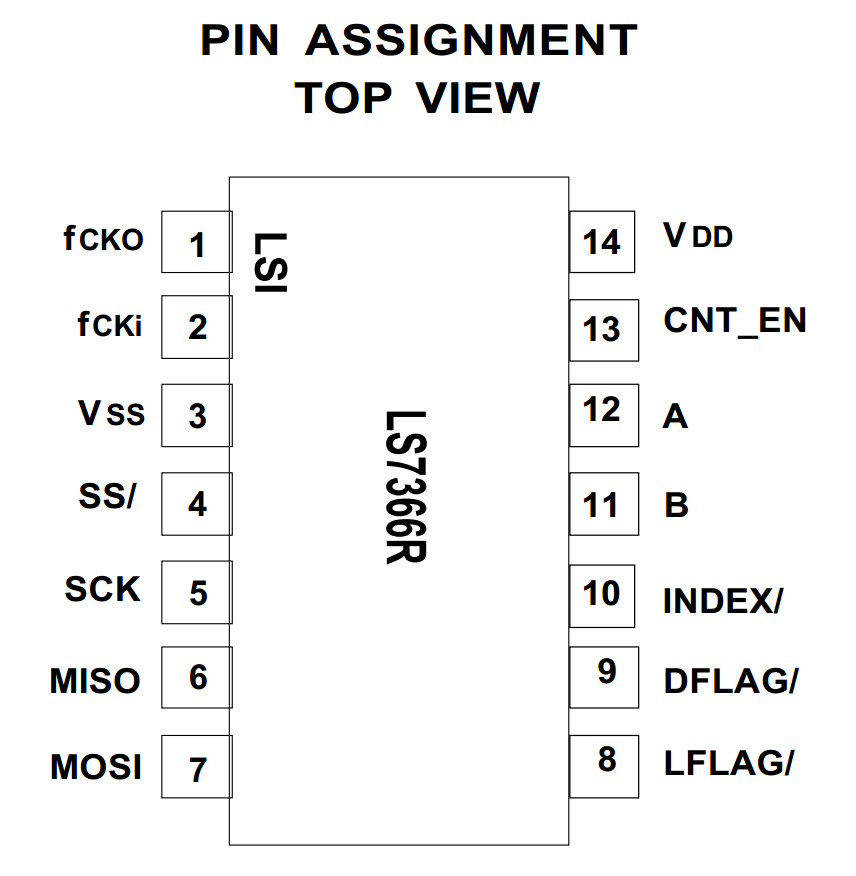
\includegraphics[scale=0.15]{images/LS7366.png} 
\caption{Diagrama de pines LS7366}
\label{fig:LS7366}
\end{figure} 

Gracias a este integrado, se evita que el microprocesador tenga que hacerse cargo del gran nombre de interupciones, permiti'endole dedicarse a otros procesos. Para la comunicaci'on se aprovecha el m'odulo propio SPI del BCM2835 y dos de los pines de selecci'on de escalvo. 

\subsubsection{Monitorizaci'on de la Bater'ia}
Conocer el estado de la bater'ia en cualquier momento es crucial en plataformas m'oviles, por ello su monitorizaje es imprescindible. Dicho monitorizaje se efectua de dos maneras distintas: La primera mediante un m'odulo ADC que digitaliza el estado de la bater'ia, y la segunda se utiliza el circuito integrado LM3914, un dispositivo encargado de medir el voltage y mostrar dicha informaci'on mediante 10 LEDs siguiendo una tendencia lineal. 


\newpage

\section{Presupuesto}
\newpage

\section{Conclusiones}
\newpage

\section{Agradecimientos}
\newpage

\section{Biografia}
\newpage

\section{Soporte inform'atico}

\end{document}